\documentclass[11pt]{article}

% ---------------------------------------------------------------------------
%  Learning concept hierarchies by compression: a tutorial research note.
%  Compiles with pdflatex + bibtex on Overleaf. Self-contained.
% ---------------------------------------------------------------------------

\usepackage[a4paper,margin=2.6cm]{geometry}
\usepackage{amsmath,amssymb}
\usepackage{booktabs}
\usepackage{xcolor}
\usepackage{tikz}
\usepackage{pgfplots}
\pgfplotsset{compat=1.17}
\usetikzlibrary{positioning,arrows.meta,fit,backgrounds,calc,shapes.geometric}
\usepackage{listings}
\usepackage[hidelinks]{hyperref}
\usepackage{microtype}

% ---- colours -----------------------------------------------------------
\definecolor{cAttr}{RGB}{70,130,180}    % attributes (steel blue)
\definecolor{cConc}{RGB}{200,120,40}     % concepts (amber)
\definecolor{cGood}{RGB}{40,140,80}      % green
\definecolor{cBad}{RGB}{190,60,60}       % red
\definecolor{cGrid}{RGB}{210,210,210}

% ---- listings ----------------------------------------------------------
\lstset{basicstyle=\ttfamily\small,breaklines=true,frame=single,
        backgroundcolor=\color{gray!6},columns=fullflexible,keepspaces=true}

% ---- handy macros ------------------------------------------------------
\newcommand{\bits}{\ \text{bits}}
\newcommand{\CL}{L}                       % codelength
\newcommand{\Shat}{\hat{S}}
\newcommand{\Yhat}{\hat{Y}}
\newcommand{\epsp}{\varepsilon^{+}}
\newcommand{\epsm}{\varepsilon^{-}}
\newcommand{\code}[1]{\texttt{#1}}

\title{\bf Learning Concept Hierarchies by Compression\\[2pt]
\large A tutorial note: from Formal Concept Analysis to a probabilistic,
minimum-description-length reworking in the spirit of Barlow's sparse codes}
\author{Peter F\"oldi\'ak}
\date{\today}

\begin{document}
\maketitle

\begin{abstract}
\noindent
Suppose you are handed a large table of yes/no facts --- which animals have
which features, which documents contain which words, which patients show which
symptoms --- and asked: \emph{what are the underlying concepts, and how do they
relate?} A classical answer, Formal Concept Analysis (FCA), builds every
concept that the data logically permits. The trouble is that real data is
noisy, and FCA faithfully invents a concept for every accidental coincidence,
producing tens of thousands of ``concepts'' where a handful were intended. This
note develops an alternative built on a single idea from information theory: a
concept is worth having exactly when positing it lets us \emph{describe the data
more briefly}. We reframe concept learning as \emph{lossy compression with a
hierarchy}, connect it to Barlow's principle that perception should remove
redundancy by recruiting a unit for each ``suspicious coincidence,'' and give a
simple greedy algorithm that recovers planted hierarchies while ignoring noise.
We report what a first prototype achieves (clean recovery of two- and
three-level hierarchies, against an FCA lattice tens of thousands of concepts
large), and we end with an honest account of a subtle limitation we uncovered
about \emph{overlapping} concepts --- one that turns out not to be a bug in the
search but a real consequence of how we price the code, and which points
directly at the next design decision.
\end{abstract}

\tableofcontents

% =======================================================================
\section{The problem}
% =======================================================================

\subsection{Binary data and the question of concepts}

Much of the world's data can be written as a grid of yes/no answers. Rows are
\emph{objects} (animals, documents, customers, cells); columns are
\emph{attributes} (features, words, purchases, active genes). A cell is $1$ if
the object has the attribute and $0$ otherwise. We call this an
object\,$\times$\,attribute \emph{context}, and write it as a matrix $X$ with
$N$ rows and $A$ columns.

\begin{figure}[h]
\centering
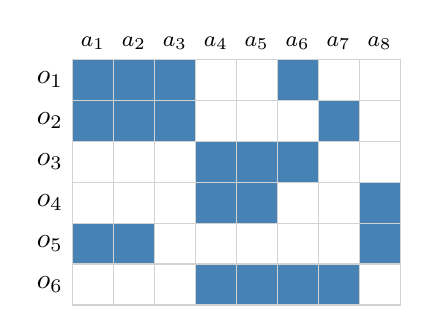
\begin{tikzpicture}[scale=0.52]
  \def\rows{6} \def\cols{8}
  % example matrix
  \foreach \r/\pat in {
     0/{1,1,1,0,0,1,0,0},
     1/{1,1,1,0,0,0,1,0},
     2/{0,0,0,1,1,1,0,0},
     3/{0,0,0,1,1,0,0,1},
     4/{1,1,0,0,0,0,0,1},
     5/{0,0,0,1,1,1,1,0}} {
    \foreach \c [count=\i from 0] in \pat {
      \pgfmathparse{\c==1 ? "cAttr" : "white"}
      \edef\col{\pgfmathresult}
      \fill[\col,draw=cGrid] (\i,-\r) rectangle ++(1,1);
    }
  }
  % labels
  \foreach \r/\name in {0/o_1,1/o_2,2/o_3,3/o_4,4/o_5,5/o_6}
     \node[left] at (0,-\r+0.5) {$\name$};
  \foreach \c/\name in {0/a_1,1/a_2,2/a_3,3/a_4,4/a_5,5/a_6,6/a_7,7/a_8}
     \node[above,rotate=0,font=\footnotesize] at (\c+0.5,1) {$\name$};
\end{tikzpicture}
\caption{A tiny binary context $X$ ($N=6$ objects, $A=8$ attributes). A filled
cell is a $1$. The eye already picks out ``blocks'': objects $o_1,o_2$ share
$a_1,a_2,a_3$; objects $o_3,o_4,o_6$ share $a_4,a_5$. Those blocks are the kind
of latent \emph{concept} we want a machine to discover --- but only the real
ones, not every accidental overlap.}
\label{fig:matrix}
\end{figure}

Given only $X$, we would like to recover a small set of \emph{concepts} ---
groups of attributes that tend to occur together for a reason --- and the
\emph{is-a} relationships among them (a \emph{penguin} is a \emph{bird} is an
\emph{animal}). Concretely we want two things:
\begin{enumerate}
  \item a compact vocabulary of concepts, each identified with the set of
        attributes it implies (its \emph{intent}), and
  \item a partial order (a hierarchy) saying which concepts specialise which.
\end{enumerate}
This is unsupervised structure learning: nobody labels the concepts; they must
be inferred from the pattern of co-occurrence alone.

\subsection{Why not just cluster, or build a tree?}

Two familiar tools fall short in instructive ways.

\emph{Clustering} assigns each object to one group. But objects genuinely
belong to several concepts at once: a tomato is a \emph{fruit} and \emph{red}
and \emph{round}. Forcing one label per object destroys exactly the
combinatorial structure we are after.

\emph{Hierarchical clustering / taxonomy trees} allow nesting but insist that
every concept has a single parent. Real concept systems are not trees: ``red''
and ``round'' are two independent axes, and ``red round thing'' sits under
\emph{both}. A structure that allows multiple parents is a \emph{directed
acyclic graph} (DAG), not a tree. Keeping the DAG generality --- and learning it
from data --- is a central goal of this project.

% =======================================================================
\section{Background: two classical answers, and one guiding principle}
% =======================================================================

\subsection{Formal Concept Analysis, and how it over-generates}

Formal Concept Analysis \cite{ganter1999} gives a beautiful, exact answer to
``what are all the concepts?''. Given the context $X$, a \emph{formal concept}
is a pair (set of objects, set of attributes) that is \emph{closed}: the objects
are exactly those having all the attributes, and the attributes are exactly
those shared by all the objects. Order the concepts by inclusion of their object
sets and you get the \emph{concept lattice} --- a complete, canonical map of
every implication in the data.

\begin{figure}[h]
\centering
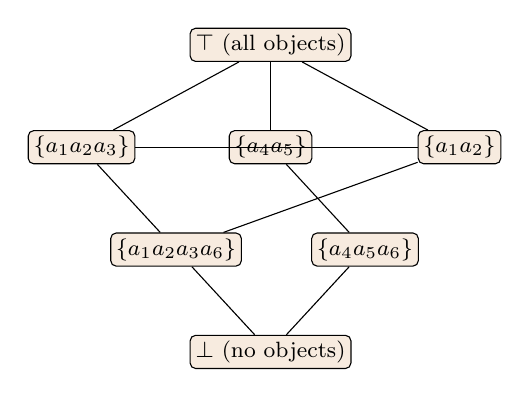
\begin{tikzpicture}[scale=1.0,every node/.style={font=\footnotesize},
    concept/.style={draw,rounded corners=2pt,fill=cConc!15,inner sep=2pt}]
  \node[concept] (top) at (0,3) {$\top$ (all objects)};
  \node[concept] (c1) at (-2.4,1.7) {$\{a_1a_2a_3\}$};
  \node[concept] (c2) at (0,1.7) {$\{a_4a_5\}$};
  \node[concept] (c3) at (2.4,1.7) {$\{a_1a_2\}$};
  \node[concept] (c4) at (-1.2,0.4) {$\{a_1a_2a_3a_6\}$};
  \node[concept] (c5) at (1.2,0.4) {$\{a_4a_5a_6\}$};
  \node[concept] (bot) at (0,-0.9) {$\bot$ (no objects)};
  \draw (top)--(c1); \draw (top)--(c2); \draw (top)--(c3);
  \draw (c3)--(c1); \draw (c1)--(c4); \draw (c2)--(c5);
  \draw (c4)--(bot); \draw (c5)--(bot); \draw (c3)--(c4);
\end{tikzpicture}
\caption{A fragment of a concept lattice for data like Figure~\ref{fig:matrix}.
Each node is a closed attribute set. On clean data this is exactly the structure
we want. The problem is what happens under noise (next).}
\label{fig:lattice}
\end{figure}

The catch is \emph{closure under intersection}. Every intersection of object
sets is itself a concept, so the number of concepts can be exponential in the
data size. Worse, this is fragile to noise. Flip a single cell --- one bird
that, by observation error, appears not to fly --- and FCA dutifully creates a
new concept ``birds that fly except this one.'' On real data with a few percent
noise, the lattice explodes into tens of thousands of concepts, almost all of
them accidents. FCA answers ``what \emph{could} be a concept?'' when we wanted
``what \emph{is} a concept?''. It has no notion that a concept should have to
\emph{earn its place}.

\subsection{Barlow: perception as redundancy reduction}

The guiding intuition for a better answer comes from neuroscience. Horace Barlow
argued \cite{barlow1961,barlow1989} that a central job of sensory coding is to
\emph{remove redundancy}: the raw signal is full of correlations (neighbouring
pixels are similar, features co-occur), and an efficient brain should re-code it
so that the resulting features are as \emph{independent} as possible --- a
\emph{factorial code}. In such a code, each recurring, statistically
\emph{suspicious} coincidence in the input is captured by a dedicated unit, so
that downstream the coincidence no longer has to be re-discovered every time.

Barlow's memorable phrasing is that the visual system should treat a
\emph{``suspicious coincidence''} --- an event far more common than chance would
predict --- as evidence for a new feature worth representing. A closely related
idea is that good sensory codes are \emph{sparse}: at any moment only a few of
many possible units are active \cite{barlow1972,foldiak1990,foldiak1995,
olshausen1996}. Sparse and factorial codes are two sides of one coin: if you
insist that few units fire and that they are informative, you are pushed towards
units that stand for genuine, reusable regularities.

This note takes Barlow's slogan literally and makes it constructive and exact:
\emph{introduce a new concept precisely when a coincidence is suspicious enough
to pay for its own description}. To make ``pay for its description'' precise we
need one more ingredient.

\subsection{Minimum Description Length: compression as model selection}

The Minimum Description Length principle \cite{rissanen1978,grunwald2007} says:
\emph{the best model of some data is the one that lets you describe the data in
the fewest bits, counting the description of the model itself}. If you must
transmit $X$ to a friend, you may first send a \emph{model} (a vocabulary of
concepts and a hierarchy) and then send $X$ \emph{using} that model. A good
model makes the second part short; a complicated model makes the first part
long. MDL picks the total-bits minimum, and this automatically penalises
over-fitting: a concept invented for one noisy coincidence costs more to
describe than it saves, so it is rejected. No significance threshold or $p$-value
is needed --- \emph{the model's own description cost is the threshold}.

MDL has a very successful incarnation in pattern mining. \textsc{Krimp}
\cite{vreeken2011} and its greedy successor \textsc{Slim} \cite{smets2012} learn
a \emph{code table}: a flat dictionary of itemsets that together compress a
transaction database. Their empirical lesson is encouraging and we lean on it
heavily: greedily considering \emph{pairwise unions of current dictionary
entries}, judged by exact change in description length, gets remarkably close to
what far more expensive global search finds.

\medskip
\noindent\textbf{The one-sentence thesis of this project.}
\emph{Take \textsc{Slim}'s ``grow a dictionary by compression'' recipe, but
replace the flat code table with a \emph{DAG of concepts with is-a (closure)
semantics}; the result is a probabilistic, MDL version of Formal Concept
Analysis that only posits a concept when it pays rent --- which is Barlow's
suspicious-coincidence unit recruitment made exact.} As far as we know the
combination (DAG-structured closure dictionary learned by MDL) is new.

% =======================================================================
\section{A quick information-theory primer}
% =======================================================================

Everything hinges on measuring bits, so here is the minimum needed, from
scratch.

\paragraph{Codelength of an event.} If an event has probability $p$, the
cheapest possible code spends $-\log_2 p$ bits on it \cite{shannon1948}.
Rare events are expensive, certain events are free. The \emph{entropy}
$H(p) = -p\log_2 p - (1-p)\log_2(1-p)$ is the average cost per symbol of the
best code for a coin that lands heads with probability $p$. It is $0$ for a
certain coin ($p\in\{0,1\}$) and maximal ($1$ bit) for a fair coin
($p=\tfrac12$). We will need one fact about $H$: it is \emph{concave} and peaks
in the middle. Splitting one column of $1$s into two moderate columns can cost
\emph{more} total entropy than the single column did --- a fact that will return
with force in Section~\ref{sec:overlap}.

\paragraph{Coding without knowing $p$ in advance.} We rarely know the true
frequency of a feature. A clean fix is the \emph{Krichevsky--Trofimov (KT)
estimator} \cite{krichevsky1981}: to code a binary sequence with $n_1$ ones and
$n_0$ zeros, predict the next bit with a running estimate that starts at
one-half and updates as
\[
  \Pr(\text{next}=1) \;=\; \frac{n_1 + \tfrac12}{\,n_1 + n_0 + 1\,}.
\]
The total bits to send the whole sequence has the closed form
\[
  \CL_{\mathrm{KT}}(n_1,n_0)
  \;=\; -\log_2 \frac{\Gamma(n_1+\tfrac12)\,\Gamma(n_0+\tfrac12)}
                     {\Gamma(\tfrac12)^2\,\Gamma(n_1+n_0+1)} .
\]
You do not need to memorise this; the point is that it is (i) parameter-free ---
the ``$+\tfrac12$'' is the only choice, and it is the principled one (a
Jeffreys/Bayes prior); and (ii) it depends only on \emph{counts}, so we can
evaluate it instantly from tallies. Because KT is a Bayesian mixture code, MDL
built on it coincides with Bayesian model selection --- a bridge we mention again
at the end.

\paragraph{Coding a whole number.} To describe the model we sometimes must send
an integer $k$ (e.g.\ ``there are $k$ concepts'') without an agreed upper bound.
Rissanen's universal code for integers \cite{rissanen1983} does this in about
$\log_2 k + \log_2\log_2 k + \cdots$ bits --- essentially ``the number of digits,
plus the digits.'' Again the detail does not matter; it is simply the honest
price of naming a concept count.

% =======================================================================
\section{The model: a concept DAG that generates noisy data}
% =======================================================================

\subsection{Structure and semantics}

Our model is a DAG with two kinds of nodes (Figure~\ref{fig:dag}):
\begin{itemize}
  \item \textbf{Attribute nodes} --- the $A$ observed columns. They are the
        \emph{sinks} (bottom) of the DAG.
  \item \textbf{Concept nodes} --- latent groupings. Each concept points to its
        \emph{children}, which may be attributes or other (lower) concepts.
\end{itemize}

\begin{figure}[h]
\centering
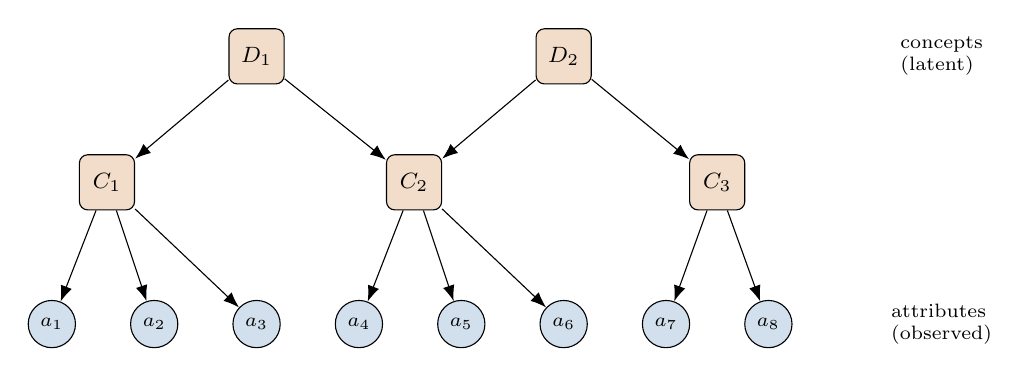
\begin{tikzpicture}[
   node distance=8mm,
   attr/.style={draw,circle,fill=cAttr!25,minimum size=6mm,inner sep=0pt,font=\scriptsize},
   con/.style={draw,rounded corners=3pt,fill=cConc!25,minimum size=7mm,inner sep=3pt,font=\footnotesize\bfseries}]
  % attributes row
  \foreach \i in {1,...,8}
    \node[attr] (a\i) at (\i*1.3,0) {$a_{\i}$};
  % base concepts
  \node[con] (B0) at (2.0,1.8) {$C_1$};
  \node[con] (B1) at (5.9,1.8) {$C_2$};
  \node[con] (B2) at (9.75,1.8) {$C_3$};
  % top concepts
  \node[con] (T0) at (3.9,3.4) {$D_1$};
  \node[con] (T1) at (7.8,3.4) {$D_2$};
  % edges concepts->attrs
  \draw[-{Latex[length=2mm]}] (B0)--(a1); \draw[-{Latex[length=2mm]}] (B0)--(a2); \draw[-{Latex[length=2mm]}] (B0)--(a3);
  \draw[-{Latex[length=2mm]}] (B1)--(a4); \draw[-{Latex[length=2mm]}] (B1)--(a5); \draw[-{Latex[length=2mm]}] (B1)--(a6);
  \draw[-{Latex[length=2mm]}] (B2)--(a7); \draw[-{Latex[length=2mm]}] (B2)--(a8);
  % edges tops->bases
  \draw[-{Latex[length=2mm]}] (T0)--(B0); \draw[-{Latex[length=2mm]}] (T0)--(B1);
  \draw[-{Latex[length=2mm]}] (T1)--(B1); \draw[-{Latex[length=2mm]}] (T1)--(B2);
  \node[font=\scriptsize,align=left] at (12.6,3.4) {concepts\\(latent)};
  \node[font=\scriptsize,align=left] at (12.6,0) {attributes\\(observed)};
\end{tikzpicture}
\caption{A concept DAG. Activating concept $D_1$ turns on everything reachable
below it: $C_1,C_2$ and hence attributes $a_1\!-\!a_6$. Note $C_2$ has
\emph{two} parents $D_1,D_2$ --- the multiple-parent structure a tree cannot
express. (This particular ``shared child'' will be the star of
Section~\ref{sec:overlap}.)}
\label{fig:dag}
\end{figure}

The semantics are \emph{deterministic downward closure}. Each object $n$ comes
with an \emph{activation set} $S_n$ of nodes it switches on. Turning on a node
turns on everything reachable from it. The predicted attribute vector $\Yhat_n$
is the union of all attributes reachable from $S_n$. Two modelling choices keep
this clean:
\begin{itemize}
  \item $S_n$ is an \emph{antichain}: we never explicitly list a node and also
        something above it (that would be redundant, since the higher node
        already implies the lower).
  \item Objects may activate a \emph{bare attribute} directly. This gives
        idiosyncratic one-off features a cheap home, so the model is not tempted
        to invent a junk concept for them.
\end{itemize}

\subsection{Where the randomness lives}

Real data is noisy, so the model includes an \emph{observation noise} layer with
two rates:
\[
  \epsp = \Pr(\text{observe }1 \mid \text{generated }0)\ \text{(false positive)},\qquad
  \epsm = \Pr(\text{observe }0 \mid \text{generated }1)\ \text{(false negative)}.
\]
The story for one object is thus: pick an antichain $S_n$; propagate closure to
get the clean prediction $\Yhat_n$; then flip each cell independently with the
appropriate small probability to get the observed row $X_n$
(Figure~\ref{fig:generate}). All stochasticity sits at this final layer; inside
the DAG, closure is exact. (Letting activation itself be probabilistic --- a
``noisy-OR'' belief network --- is a deliberate future extension, discussed at
the end.)

\begin{figure}[h]
\centering
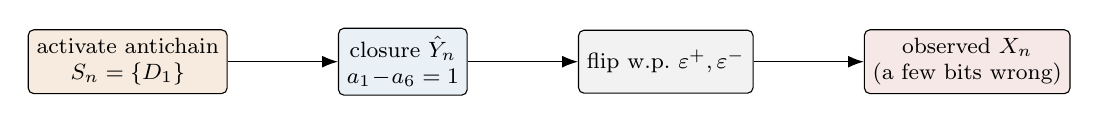
\begin{tikzpicture}[node distance=6mm,font=\footnotesize,
   box/.style={draw,rounded corners=2pt,minimum height=8mm,align=center,inner sep=3pt}]
  \node[box,fill=cConc!15] (s) {activate antichain\\ $S_n=\{D_1\}$};
  \node[box,fill=cAttr!12,right=14mm of s] (y) {closure $\Yhat_n$\\ $a_1\!-\!a_6=1$};
  \node[box,fill=gray!10,right=14mm of y] (x) {flip w.p.\ $\epsp,\epsm$};
  \node[box,fill=cBad!12,right=14mm of x] (o) {observed $X_n$\\ (a few bits wrong)};
  \draw[-{Latex[length=2mm]}] (s)--(y);
  \draw[-{Latex[length=2mm]}] (y)--(x);
  \draw[-{Latex[length=2mm]}] (x)--(o);
\end{tikzpicture}
\caption{The generative process for a single object. Learning inverts this:
from many observed rows $X_n$, recover the DAG and the (hidden) activations.}
\label{fig:generate}
\end{figure}

\subsection{The total codelength}

The description we must minimise has three parts:
\begin{equation}
\CL(G,X)\;=\;\underbrace{\CL(G)}_{\text{structure}}
\;+\;\underbrace{\textstyle\sum_n \CL(S_n\mid G)}_{\text{usage}}
\;+\;\underbrace{\textstyle\sum_n \CL(X_n\mid S_n,G)}_{\text{residual}} .
\label{eq:decomp}
\end{equation}

\paragraph{Structure $\CL(G)$.} The price of the map itself: how many concepts
(a Rissanen integer code), and which edges exist (coded with a single global KT
Bernoulli, so a dense DAG makes each edge cheap and a sparse one makes each edge
dear --- adaptive, nothing hand-tuned).

\paragraph{Usage $\CL(S_n\mid G)$ --- the rent.} For each dictionary item
$k$ (concept or bare attribute) we code the column ``is $k$ explicitly active in
object $n$?'' across all objects, with a per-item KT Bernoulli. \emph{This is the
term that makes concepts pay rent.} A concept used by many objects gets a cheap
per-use price and is a bargain; a concept used once costs almost as much as
spelling out its attributes raw, so it dies. This is precisely the mechanism FCA
lacks.

\paragraph{Residual $\CL(X_n\mid S_n,G)$.} The corrections: the false positives
and false negatives between the prediction $\Yhat_n$ and the observation $X_n$,
coded with KT-estimated $\epsp,\epsm$.

MDL now selects the DAG minimising the sum \eqref{eq:decomp}. Three degenerate
extremes are automatically punished, which is a good sanity check:
\begin{center}
\begin{tabular}{lll}
\toprule
Model & structure $\CL(G)$ & residual \\
\midrule
Full FCA lattice (a concept per coincidence) & enormous & zero \\
One concept per distinct object & enormous & zero \\
Empty model (no concepts) & zero & enormous \\
\bottomrule
\end{tabular}
\end{center}
The good ontology lives in the valley between them.

% =======================================================================
\section{The key identity: ``correlation'' \emph{is} change-in-codelength}
% =======================================================================

Here is the bridge from Barlow's slogan to a concrete algorithm. Suppose we are
considering creating a concept $c$ that stands for the co-occurrence of two
existing dictionary items $a$ and $b$. Let $n_{ab}$ be the number of objects
that currently use \emph{both}. Introducing $c$ and rewriting those objects to
use $c$ instead of $a\!+\!b$ changes the total codelength by approximately
\begin{equation}
\Delta \CL \;\approx\; -\,n_{ab}\,\big[\,\underbrace{-\log_2 \hat q_a - \log_2\hat q_b + \log_2 \hat q_c}_{\text{bits saved per shared use}}\big]\;+\;\text{overhead},
\label{eq:delta}
\end{equation}
where $\hat q_{\bullet}$ are the KT-estimated usage frequencies and the overhead
is the structure bits for the new node and its edges, plus the new usage column,
\emph{plus a subtle re-pricing of $a$ and $b$ whose own usage frequencies drop
once $c$ absorbs their joint occurrences}. To first order this is
\[
  \Delta\CL \;\approx\; -\,N\cdot I(a;b)\;+\;\text{overhead},
\]
where $I(a;b)$ is the \emph{mutual information} between the two items: their
statistical dependence, weighted by how much data we have. In words:

\begin{quote}
\emph{The number of bits a new concept saves is the strength of the coincidence
it captures, times the amount of evidence for it, minus the cost of writing the
concept down.}
\end{quote}

This is exactly Barlow's ``suspicious coincidence,'' quantified. ``Add the
strongest correlation'' and ``take the most compressive MDL step'' are the
\emph{same move}; the MDL form simply gets the acceptance threshold and the
tie-breaking right for free, and --- crucially --- includes the re-pricing term
that na\"ive correlation scores miss.

% =======================================================================
\section{The algorithm: grow a DAG by greedy pair-merging}
% =======================================================================

\subsection{The main loop}

We start from the simplest possible model --- no concepts, every object coded by
its raw attributes --- and repeatedly add the single most profitable concept.

\begin{lstlisting}
initialise: dictionary = attributes only; each object's code = its 1s
repeat:
    rank candidate pairs (a,b) by a cheap upper bound on their saving
        (bound = n_ab * pointwise-mutual-information)
    take the best candidate; compute its EXACT change-in-codelength dL
        (evaluate lazily: only re-check the top few, since gains
         almost only shrink as the dictionary grows -- a safe shortcut)
    if dL < 0 (it compresses):
        create concept c = {a,b}
        re-encode ONLY the objects that used both a and b (use an index)
        update the counts
    every few accepts: PRUNE-AND-COLLAPSE weak or redundant concepts
until no candidate compresses
\end{lstlisting}

Three points deserve unpacking.

\paragraph{Everything is a count.} The score \eqref{eq:decomp} and every
$\Delta\CL$ depend only on tallies: how often each item is used, how often each
pair is co-used, and the residual error totals. We keep these in a
\emph{counter store} and the scorer talks \emph{only} to it, never re-scanning
the raw data. This is what makes each candidate evaluation $O(1)$ instead of
$O(N)$, and it is the design commitment that later lets the same code run in a
streaming/online mode.

\paragraph{Explaining away comes for free.} We track co-occurrence in the
\emph{current code} $S_n$, not in the raw data. The moment $c=\{a,b\}$ is
created and absorbs their joint uses, the residual co-occurrence of $a$ and $b$
collapses, so we never re-propose it --- and \emph{new} correlations involving
$c$ itself become visible. That is precisely how the hierarchy climbs: pairs of
base concepts become the children of a mid concept, pairs of mids become the
children of a top.

\paragraph{Devaluation and the pruning sweep.} A five-attribute concept gets
built as a \emph{ladder} of binary merges, and the intermediate rungs are often
used \emph{only} inside the bigger concept above them. A periodic sweep asks of
each concept: if I delete it and re-route its uses to its children, does the
total shrink? If so, collapse it. Without this the dictionary silts up with dead
rungs.

\subsection{One thing we had to add: escaping the ``no-noise'' trap}

We found, and fixed, a subtle failure. Early in learning the model is perfect on
the (still-uncompressed) data --- zero residual error. Under the KT code, the
\emph{first} false negative is very expensive (its estimated rate is near zero,
so admitting one costs $\sim$$15$ bits), so no single object will ever
volunteer to adopt a concept-plus-noise encoding, even though a whole
\emph{cohort} of similar objects doing so together is cheap. The learner gets
stuck coding noise via junk concepts. Our fix is a \emph{batch re-encoding}
step: periodically re-encode \emph{all} objects at once using a few trial noise
rates, and accept the whole pass only if the exact global codelength drops. The
trial rates are just a proposal device; acceptance is still the one true score,
so no threshold sneaks into the model. This is worth flagging because it will
recur in any MDL learner with a costly ``first error'': the escape has to be
collective, not per-object.

% =======================================================================
\section{Results so far}
% =======================================================================

We validate on \emph{planted} data: we build a known hierarchy, sample objects
from it with $2\%$ noise, hand the learner only $X$, and ask whether it recovers
the hierarchy and beats the description length of the very model that generated
the data.

\subsection{Compression trajectory}

\begin{figure}[h]
\centering
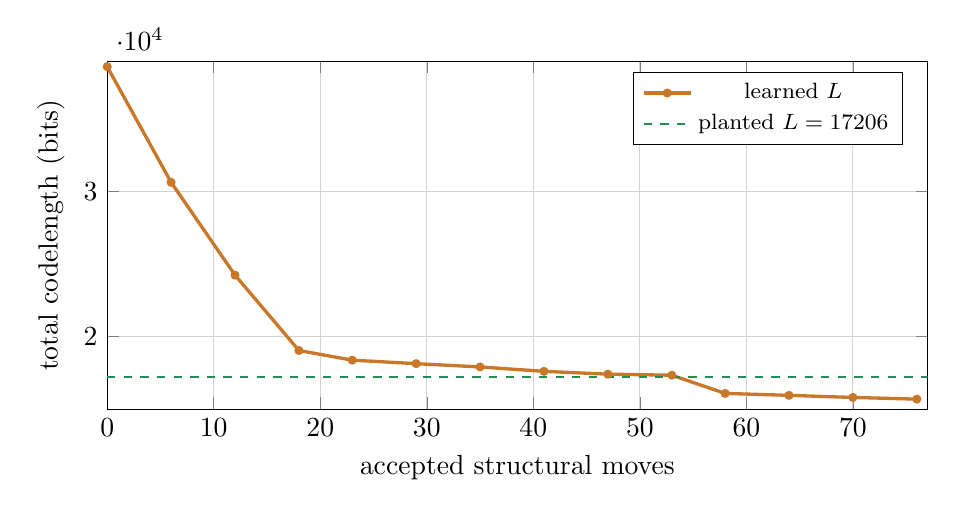
\begin{tikzpicture}
\begin{axis}[width=12cm,height=6cm,
    xlabel={accepted structural moves},
    ylabel={total codelength (bits)},
    ymin=15000,ymax=39000, xmin=0,xmax=77,
    grid=both, grid style={cGrid},
    legend pos=north east, legend style={font=\footnotesize}]
  \addplot[cConc,very thick,mark=*,mark size=1pt] coordinates {
    (0,38623)(6,30644)(12,24241)(18,19042)(23,18377)(29,18135)(35,17908)
    (41,17605)(47,17410)(53,17338)(58,16082)(64,15949)(70,15804)(76,15688)};
  \addlegendentry{learned $\CL$}
  \addplot[cGood,dashed,thick,domain=0:77] {17206};
  \addlegendentry{planted $\CL=17206$}
\end{axis}
\end{tikzpicture}
\caption{The learner's total codelength as it adds concepts, on a planted
two-level hierarchy ($A=20$ attributes, $6$ concepts, $N=2000$ objects,
$2\%$ noise). Every accepted move provably decreases the score (we assert
this). The final model is \emph{shorter} than the planted one (green line):
having seen the noise, the learner codes it slightly more efficiently than the
generating model does on its own sample.}
\label{fig:traj}
\end{figure}

\subsection{Recovery quality}

\begin{table}[h]
\centering
\begin{tabular}{lccccc}
\toprule
planted hierarchy & concepts recovered & extent Jaccard & order P/R & $\CL$ ratio & FCA lattice size \\
\midrule
2 levels ($A{=}20$, $K{=}6$)  & $6/6$   & $\ge 0.99$ & $1.00/1.00$ & $0.91$ & $57\,000+$ \\
3 levels ($A{=}30$, $K{=}14$) & $14/14$ & $\ge 0.96$ & $1.00/1.00$ & $0.92$ & (explodes) \\
\bottomrule
\end{tabular}
\caption{Planted-recovery results. \emph{Extent Jaccard}: overlap between each
planted concept's set of objects and its best-matching learned concept
($1.0$ = identical). \emph{Order P/R}: precision and recall of the learned
is-a relation against the planted partial order. \emph{$\CL$ ratio}:
learned\,/\,planted codelength ($<1$ = the learner compresses better than the
generator). \emph{FCA lattice size}: number of closed sets a classical FCA would
report on the same noisy data --- the ``what we saved you from'' number.}
\label{tab:recovery}
\end{table}

The headline is the last two columns of Table~\ref{tab:recovery} read together:
where classical FCA reports \emph{tens of thousands} of concepts on this noisy
data, our method reports the \emph{six} (or fourteen) that pay rent, recovers
them essentially exactly, and does so while describing the data in fewer bits
than the true generator uses. The three-level result matters especially: it
shows that depth \emph{builds on depth} --- mid-level concepts are discovered
from the co-occurrence of already-learned base concepts, and top concepts from
the co-occurrence of already-learned mids --- using nothing but repeated pairwise
merging.

% =======================================================================
\section{An honest limitation: overlapping concepts}
\label{sec:overlap}
% =======================================================================

Here is where the story gets interesting, and where we spent this round of work.
All the successes above share a feature: the planted concepts have
\emph{disjoint} children. Each attribute belongs to one base concept; each base
belongs to one parent. What happens when concepts genuinely \emph{overlap} ---
when one concept is a child of two different parents (the shared $C_2$ in
Figure~\ref{fig:dag})? A tomato is both a fruit and a red-round-thing;
``edible'' might sit under both. Overlap is the whole reason we wanted a DAG
rather than a tree, so this is not a corner case --- it is the point.

\subsection{The tempting argument, and the experiment that refuted it}

One hopes overlap simply ``drops out'' of the principles: a shared child is just
a coincidence used by two parents; surely compression handles it. We tested this
directly. We planted the DAG of Figure~\ref{fig:dag} --- two top concepts
$D_1=\{C_1,C_2\}$ and $D_2=\{C_2,C_3\}$ sharing the middle base $C_2$ --- sampled
$5000$ noisy objects with the tops as the dominant generators, and ran the
\emph{unchanged} learner.

The result was sharp and, at first, disappointing:
\begin{itemize}
  \item The three base concepts $C_1,C_2,C_3$ were recovered \emph{perfectly}
        (Jaccard $1.00$).
  \item \emph{Neither} top concept was recovered.
  \item The learner's codelength was \emph{far below} the planted model's
        (ratio $\approx 0.87$).
\end{itemize}
That last point is the tell. The learner is not failing to search --- it is
\emph{correctly} finding that, under our current score, the flat three-base model
is genuinely cheaper than the intended five-node hierarchy. When we asked the
scorer directly what it would cost to add the true top $D_1=\{C_1,C_2\}$ at the
learned solution, the answer was $\mathbf{+3051}$ \textbf{bits} --- a large
\emph{increase} --- despite $C_1$ and $C_2$ co-occurring $1607$ times out of
$5000$. Why?

\subsection{Why a shared child cannot pay rent --- the concavity of entropy}

Recall that with deterministic closure, an intermediate concept changes
\emph{nothing} about the prediction (the base concepts already predict their
attributes exactly). So the residual term does not move at all. The \emph{only}
effect of adding $D_1$ is on the \emph{usage} columns --- and there it is forced
to turn \emph{two} columns into \emph{three}:

\begin{figure}[h]
\centering
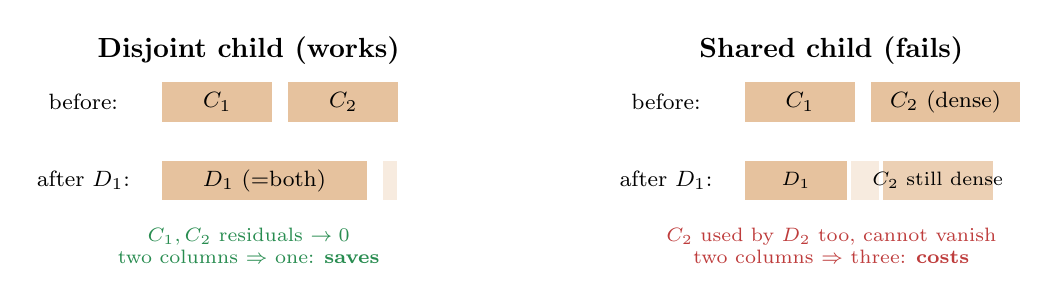
\begin{tikzpicture}[font=\footnotesize]
 % ---- disjoint case ----
 \begin{scope}
   \node[font=\bfseries] at (2.1,3.2) {Disjoint child (works)};
   % before
   \node at (0.0,2.55) {before:};
   \fill[cConc!45] (1.0,2.3) rectangle ++(1.4,0.5); \node at (1.7,2.55) {$C_1$};
   \fill[cConc!45] (2.6,2.3) rectangle ++(1.4,0.5); \node at (3.3,2.55) {$C_2$};
   % after
   \node at (0.0,1.55) {after $D_1$:};
   \fill[cConc!45] (1.0,1.3) rectangle ++(2.6,0.5); \node at (2.3,1.55) {$D_1$ (=both)};
   \fill[cConc!15] (3.8,1.3) rectangle ++(0.18,0.5);
   \node[font=\scriptsize,align=center,text=cGood] at (2.1,0.72)
        {$C_1,C_2$ residuals $\to 0$\\ two columns $\Rightarrow$ one: \textbf{saves}};
 \end{scope}
 % ---- shared case ----
 \begin{scope}[xshift=7.4cm]
   \node[font=\bfseries] at (2.1,3.2) {Shared child (fails)};
   \node at (0.0,2.55) {before:};
   \fill[cConc!45] (1.0,2.3) rectangle ++(1.4,0.5); \node at (1.7,2.55) {$C_1$};
   \fill[cConc!45] (2.6,2.3) rectangle ++(1.9,0.5); \node at (3.55,2.55) {$C_2$ (dense)};
   \node at (0.0,1.55) {after $D_1$:};
   \fill[cConc!45] (1.0,1.3) rectangle ++(1.3,0.5); \node[font=\scriptsize] at (1.65,1.55) {$D_1$};
   \fill[cConc!15] (2.35,1.3) rectangle ++(0.35,0.5); \node[font=\scriptsize] at (2.52,1.05){\,};
   \fill[cConc!35] (2.75,1.3) rectangle ++(1.4,0.5); \node[font=\scriptsize] at (3.45,1.55) {$C_2$ still dense};
   \node[font=\scriptsize,align=center,text=cBad] at (2.1,0.72)
        {$C_2$ used by $D_2$ too, cannot vanish\\ two columns $\Rightarrow$ three: \textbf{costs}};
 \end{scope}
\end{tikzpicture}
\caption{Why disjoint concepts pay rent and shared ones do not, in terms of
usage columns (width $\propto$ how many objects explicitly use the item).
\emph{Left:} when $C_1,C_2$ belong only to $D_1$, creating $D_1$ empties their
columns --- two columns become one. \emph{Right:} when $C_2$ is shared with
another parent $D_2$, its column stays dense no matter what $D_1$ does --- so we
have simply \emph{added} a third column.}
\label{fig:columns}
\end{figure}

Now use the concavity of entropy. Writing $u/N$ for a column's density, its cost
is about $N\cdot H(u/N)$ bits. In the shared experiment the numbers were:
\[
  \text{before:}\quad N\big[H(0.45)+H(0.73)\big]\approx 9160\bits,
  \qquad
  \text{after:}\quad N\big[H(0.13)+H(0.41)+H(0.32)\big]\approx 12190\bits.
\]
The total number of $1$s actually went \emph{down} (the shared uses are no
longer double-counted), yet the cost went \emph{up} by $\sim 3000$ bits, because
splitting into a third moderate-density column adds entropy faster than the
removed $1$s save it. Figure~\ref{fig:entropy} shows the geometry: three points
partway up the hump sum higher than two.

\begin{figure}[h]
\centering
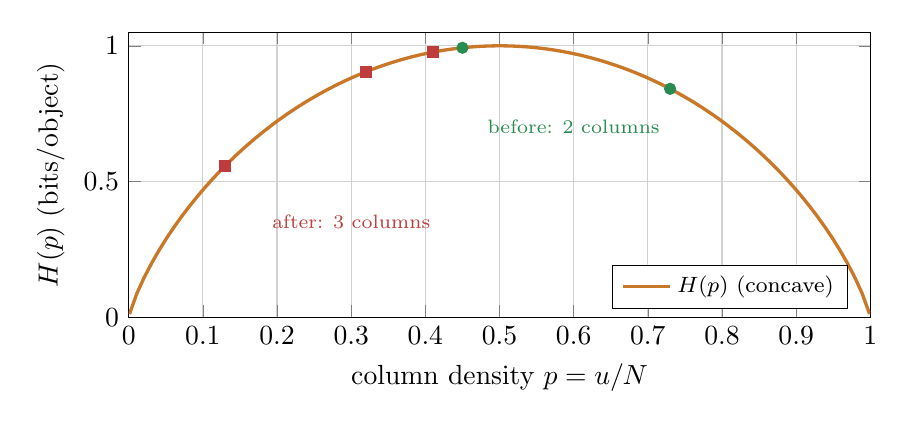
\begin{tikzpicture}
\begin{axis}[width=11cm,height=5.2cm,
   xlabel={column density $p=u/N$}, ylabel={$H(p)$ (bits/object)},
   domain=0.001:0.999, samples=100, ymin=0,ymax=1.05,xmin=0,xmax=1,
   grid=both,grid style={cGrid},legend pos=south east,legend style={font=\footnotesize}]
  \addplot[cConc,very thick]{-x*log2(x)-(1-x)*log2(1-x)};
  \addlegendentry{$H(p)$ (concave)}
  % before points (green)
  \addplot[only marks,mark=*,cGood,mark size=2pt] coordinates {(0.45,0.9928)(0.73,0.8415)};
  % after points (red)
  \addplot[only marks,mark=square*,cBad,mark size=2pt] coordinates {(0.13,0.5574)(0.41,0.9765)(0.32,0.9044)};
  \node[cGood,font=\scriptsize] at (axis cs:0.60,0.70) {before: 2 columns};
  \node[cBad,font=\scriptsize]  at (axis cs:0.30,0.35) {after: 3 columns};
\end{axis}
\end{tikzpicture}
\caption{Entropy is concave. Two moderately dense columns (green circles, sum
$\approx 1.83$) become three columns of middling density (red squares, sum
$\approx 2.44$) when a shared child is factored out --- \emph{more} total cost
even though fewer $1$s are stored. This, not a search failure, is why the
current model refuses overlapping concepts.}
\label{fig:entropy}
\end{figure}

By contrast, when the child is \emph{not} shared (Figure~\ref{fig:columns},
left) its residual column drops to zero and two columns genuinely become one ---
so the disjoint hierarchies of the previous section pay rent easily. We
confirmed this too: the same experiment with disjoint parents recovers
\emph{all} concepts perfectly.

\subsection{The real diagnosis --- and it is a feature, not a bug}

The mistake in the tempting argument was to treat the usage columns as
\emph{independent}. They are not: an object uses $D_1$, \emph{or} it uses $C_1$
and $C_2$ separately, but rarely both --- the parent and its children's residual
columns are strongly \emph{anti}-correlated. Our per-item code prices each column
as if the items were independent Bernoulli variables, and so it \emph{double
pays} whenever they are dependent. For disjoint structure the closure DAG can
actually make the explicit activations near-independent (that is what
compression is doing), and the independent-column price is right. For overlapping
structure, no pure closure code can make the activations independent, and the
independent-column price penalises the sharing that a DAG is supposed to exploit.

This is a genuinely satisfying diagnosis because it lands us right back on
Barlow. The ideal code is \emph{factorial}: its units fire independently. Our
usage term is only \emph{correct} when we have reached that ideal. Tree-like
(disjoint) hierarchies can reach it; overlapping ones cannot, under closure
semantics with an independent-column code. The learner refusing an overlapping
concept is the score honestly reporting ``this concept does not make your code
more factorial.''

% =======================================================================
\section{Open questions and design decisions}
% =======================================================================

The overlap finding sharpens the central open question rather than blocking
progress. In rough priority order:

\paragraph{1. How should usage be coded so that sharing can pay?}
This is the decision the rest depends on. Three candidate directions:
\begin{itemize}
  \item \textbf{Conditional (DAG-aware) usage coding.} Code a node's activation
        \emph{conditional on its parents}: $\Pr(\text{child active}\mid
        \text{parent active})$. This captures the anti-correlation exactly and
        should let a shared child pay rent. It is a small change to the counter
        store (condition the tallies on parent state) but it complicates the
        acyclic bookkeeping.
  \item \textbf{Noisy-OR propagation} (roadmap item, see below): replace
        deterministic closure with probabilistic activation down the edges. A
        shared child then has a real generative role and the independence
        assumption is relaxed at the source. This is the most principled and the
        most work.
  \item \textbf{Accept the scope.} Declare that v1 learns the ``tree-like
        backbone'' of a concept system and treat overlap as a second-stage
        refinement. Cheapest, least satisfying, but a legitimate staging.
\end{itemize}
Our current lean is towards conditional usage coding as the smallest change that
restores the principle, with noisy-OR as the eventual home.

\paragraph{2. Richer proposals than pair-merge.} Pairwise merging is blind to
purely higher-order structure (dependencies with no pairwise signal --- a
non-issue for is-a data, but worth stating). Planned additions: an
\emph{add-edge} move ($k\to j$ when $j$ is active in most objects using $k$),
which refactors a shared attribute \emph{upward} into a parent and is the natural
way to \emph{discover} overlap rather than merely price it; \emph{split} and
\emph{merge} moves; and mining candidate concepts from the closed itemsets of the
current \emph{residual}.

\paragraph{3. Online / streaming version.} Because the score is entirely
count-based, the same machinery runs on a stream: decay the counts, update per
object, never look back. This is \emph{prequential} MDL \cite{dawid1984} and, in
neural terms, a Hebbian coincidence detector with an MDL recruitment threshold
--- arguably the most faithful computational reading of Barlow's proposal.

\paragraph{4. Bayesian version, nearly for free.} Because KT codes are Bayesian
mixtures, our MDL score is already approximately a negative log
marginal-likelihood. Running Metropolis at temperature $1$ over the same
proposals samples an approximate \emph{posterior} over DAGs --- useful for
reporting uncertainty in the recovered structure.

\paragraph{5. Deep, fully generative version.} The long-term target replaces
deterministic closure with stacked noisy-OR layers and an unbounded
nonparametric structure prior (a cascading Indian Buffet Process
\cite{adams2010}; relatives include multiple-cause models \cite{saund1995}).
Whether learned codes \emph{stay} downward-closed under free propagation is an
empirical question we intend to measure rather than assume.

\paragraph{6. Baselines and real data.} For a proper evaluation we will compare
against flat MDL pattern miners (\textsc{Krimp}/\textsc{Slim}
\cite{vreeken2011,smets2012}), Boolean matrix factorisation with MDL model
selection \cite{miettinen2008,miettinen2011}, and the correlation-explanation
approach CorEx \cite{versteeg2014}, and move from planted data to
taxonomy-annotated real contexts --- and eventually to binarised sparse neural
codes, closing the loop to the original motivation: reading a learned sparse
representation \emph{as} an ontology.

% =======================================================================
\section*{Summary}
% =======================================================================
\addcontentsline{toc}{section}{Summary}

We set out to learn concept hierarchies from noisy binary data without FCA's
combinatorial explosion. The organising idea is old and simple --- Barlow's
suspicious coincidence --- made exact through minimum description length: posit a
concept exactly when it shortens the total description, evaluate that saving
$O(1)$ from counts, and let the model cost be the only threshold. A greedy
pair-merging learner recovers planted two- and three-level hierarchies cleanly,
compressing better than the generating model where classical FCA would report
tens of thousands of spurious concepts. Investigating overlapping concepts
turned up a clean, principled limitation --- an independent-column usage code
cannot reward a shared child, because entropy is concave and the shared child's
column never empties --- which is not a search failure but the score correctly
reporting that overlap does not make the code more factorial. That diagnosis
names the next design decision precisely: teach the usage code about the DAG's
own dependence, and the sharing a hierarchy exists to exploit will finally pay
its rent.

\bibliographystyle{plain}
\bibliography{refs}

\end{document}
